%------------------------------------------------------------------------------
% master.tex
%
% This file contains all the directive to include the different
% part of the document and build it during the compilation
% phase.
%
% To compile correctly the entire document follow these
% commands in a shell positioned in the folder that contains
% the master document (master.tex):
%
%		1) pdflatex -output-directory cover/ cover/cover.tex
%		2) pdflatex -output-directory cover/ cover/cover-frn.tex
%		3) pdflatex -output-directory cover/ cover/cover.tex
%		4) pdflatex master
%   	5) makeglossaries master
%		6) pdflatex master
%		7) pdflatex master
%------------------------------------------------------------------------------
%------------------------------------------------------------------------------
% preamble.tex
%
% Contains the document preamble with the inclusion of the
% necessary packages necessary to build correctly the final
% document.
%------------------------------------------------------------------------------
\documentclass[paper=A4, fontsize=11pt, parskip=full]{scrreprt}

\usepackage{acronym}
\usepackage{graphicx}
\usepackage{ifthen}
\usepackage{lastpage}
\usepackage{longtable}
\usepackage{multirow}
\usepackage{pdfpages}
\usepackage{sectsty}
\usepackage{siunitx}
\usepackage[utf8]{inputenc}
\usepackage[babel]{csquotes}
\usepackage[T1]{fontenc}
\usepackage[hyphens]{url}
\usepackage[hidelinks]{hyperref}
\usepackage[english, italian]{babel}
\usepackage[nonumberlist, toc]{glossaries}
\usepackage[protrusion=true, expansion=true]{microtype}
\usepackage[automark, headsepline, footsepline, markuppercase]{scrpage2}

\allsectionsfont{\centering\normalfont\scshape}

\pagestyle{scrheadings}

\lehead{Sistemi Concorrenti e Distributi}
\rohead{Simulatore di traffico}
\chead{}
\cfoot{\thepage{} di \pageref{LastPage}}

\setglossarystyle{altlist}
\makeglossaries

\newcommand{\english}[1]{\foreignlanguage{english}{\textit{#1}}}
\newcommand{\keyword}[1]{\textbf{#1}}
\newcommand{\printTOC}[1]{\ifthenelse{\equal{#1}{TRUE}}{\tableofcontents{}}{}}
\newcommand{\printTOF}[1]{\ifthenelse{\equal{#1}{TRUE}}{\listoffigures{}}{}}
\newcommand{\printTOT}[1]{\ifthenelse{\equal{#1}{TRUE}}{\listoftables{}}{}}
\newcommand{\printGLO}[1]{\ifthenelse{\equal{#1}{TRUE}}{\printglossary[title=Glossario]{}}{}}
\newcommand{\glossarySng}[1]{\underline{\gls{#1}}}
\newcommand{\glossaryPlr}[1]{\underline{\glspl{#1}}}

%------------------------------------------------------------------------------
% acronymDatabase.tex
%
% This file contains the acronym that are present in tthe
% document.
%------------------------------------------------------------------------------

%------------------------------------------------------------------------------
% glossaryDatabase.tex
%
% This file contains the terms that are present in the glossary
% at the end of the document.
%------------------------------------------------------------------------------

\begin{document}

% Document cover
\includepdf[pages={1}]{cover.pdf}
\clearpage{}

\mbox{}
\thispagestyle{empty}
\newpage

%------------------------------------------------------------------------------
% abstract.tex
%
% This illustrates brief notes about the report
%------------------------------------------------------------------------------
\section*{Note su questo report}
\label{note_su_questo_report}
Quest'opera è distribuita con licenza \english{Creative} \english{Commons} Attribuzione - Non commerciale - Condividi allo stesso modo 3.0 \english{Unported}. Un riassunto in linguaggio accessibile a tutti della Licenza in version 3.0 è reperibile all'indirizzo \url{http://creativecommons.org/licenses/by-nc-sa/3.0/}.

Tu sei libero di:
\begin{itemize}
\item{\keyword{CONDIVIDERE}: riprodurre, distribuire, comunicare al pubblico, esporre in pubblico, rappresentare, eseguire e recitare questo materiale con qualsiasi mezzo e formato}
\item{\keyword{MODIFICARE}: remixare, trasformare il materiale e basarti su di esso per le tue opere}
\end{itemize}
alle seguenti condizioni:

\keyword{ATTRIBUZIONE}: devi attribuire la paternità di quest'opera nei modi indicati dall'autore o da chi ti ha fornito l'opera in licenza ed in modo tale da non suggerire che essi avallino te o il modo in cui usi l'opera.

\keyword{NON COMMERCIALE}: non puoi utilizzare il materiale per scopi commerciali.

\keyword{STESSA LICENZA}: se remixi, trasformi il materiale o ti basi su di esso, devi distribuire i tuoi contenuti con la stessa licenza del materiale originario. 

Il licenziante non piò revocare questi diritti fintanto che tu rispetti i termini della licenza sopra citata.

\begin{figure}[h]
\centerline{
\includegraphics[scale=0.3]{images/abstract/cc-by-nc-sa.png}}
\end{figure}

\subsection*{Colophon}
\label{colophon}
Lo sviluppo di questo documento, e del progetto a cui fa riferimento, sono gestiti mediante un \english{repository} Git disponibile al seguente indirizzo \url{https://bitbucket.org/meneghinello-andrea/scd-city-web-application}.

E' possibile scaricare un archivio compresso con il codice sorgente dell'ultima versione disponibile del progetto al seguente indirizzo \url{https://bitbucket.org/meneghinello-andrea/scd-city-web-application}

% Document indexes
\printListOfContents{TRUE}
\printListOfFigures{TRUE}
\printListOfTables{TRUE}
%\clearpage{}

% Document chapters
%------------------------------------------------------------------------------
% introduction.tex
%
% This  chapter describe the problem that the canditate must
% resolve in order to participate in final examination and the
% problematics that he encountered during the desing and the
% development.
%------------------------------------------------------------------------------
\chapter*{introduzione}
\addcontentsline{toc}{chapter}{Introduzione}
\label{introduzione}
Il presente documento contiene le considerazioni finali, tratte dallo studente, in merito al progetto relativo al Corso di Sistemi Concorrenti e Distribuiti seguito durante l'anno accademico 2014-2015 presso l'Università degli Studi di Padova. Il progetto ha lo scopo di far acquisire le abilità nel risolvere problematiche utilizzando le tecniche di base della \keyword{concorrenza} e della \keyword{distribuzione}

\section*{il problema affrontato}
\addcontentsline{toc}{section}{Il problema affrontato}
\label{introduzione-il-problema-affrontato}
Al termine del corso è stata richiesta, da parte del docente, la progettazione e la conseguente realizzazione di un simulatore di traffico cittadino.

Il sistema, oggetto della relazione, è composto da:

\begin{itemize}
\item{una città  configurabile prima dell'avvio del sistema;}
\item{un insieme configurabile di persone che, in simultanea, svolgono le proprie mansioni all'interno della città;}
\item{un insieme configurabile di veicoli che, in simultanea, sono in grado di trasportare le persone a specifici indirizzi all'interno della città; Il sistema deve possedere almeno i seguenti mezzi di locomozione:}
\begin{itemize}
\item{autobus;}
\item{automobili;}
\item{pedoni.}
\end{itemize}
\item{una componente di monitoraggio che consenta all'operatore di poter essere a conoscenza della stato attuale della simulazione.}
\end{itemize}

Al fine di rendere l'esperienza di utilizzo del simulatore più funzionale e gradevole, si è corredato il sistema di:

\begin{itemize}
\item{una componente grafica che permetta la visualizzazione della simulazione da più computer contemporaneamente;}
\item{una componente che sia in grado di configurare un eseguibile, in grado di lanciare l'intero sistema, secondo le esigenze configurate dal sistemista.}
\end{itemize}

\section*{struttura del documento}
\addcontentsline{toc}{section}{Struttura del documento}
\label{introduzione-struttura-del-documento}
Il seguente documento è stato cosi suddiviso in capitoli:

\begin{enumerate}
\item{\keyword{problematiche}: capitolo in cui sono illustrate le problematiche riscontrate durante la fase di progettazione del sistema;}
\item{\keyword{analisi della soluzione}: capitolo in cui viene eseguita una analisi della soluzione proposta;}
\item{\keyword{soluzione proposta}: capitolo in cui viene illustrata la soluzione;}
\item{\keyword{conclusioni}: capitolo in cui si sono tratte delle considerazioni finali.}
\end{enumerate}

\section*{convenzioni tipografiche}
\addcontentsline{toc}{section}{Convenzioni tipografiche}
\label{introduzione-convenzioni-tipografiche}
Nel seguente documento si sono rispettate le seguenti convenzioni tipografiche:

\begin{itemize}
\item{\keyword{grassetto}: per i termini rilevanti all'interno del paragrafo;}
\item{\english{corsivo}: per i termini in lingua inglese.}
\end{itemize}
%______________________________________________________________________________
% issues.tex
%
% This illustrates the project's issues.
%______________________________________________________________________________
\chapter*{problematiche}
\addcontentsline{toc}{chapter}{Problematiche}
\label{problematiche}
In questa sezione del documento sono illustrati i problemi riscontrati durante l'analisi del sistema richiesto. Tali problematiche sono derivanti dalla tipologia del sistema e dai requisiti esplicitati.

\section*{tipologia del simulatore}
\addcontentsline{toc}{section}{Tipologia del simulatore}
\label{problematiche_tipologia_del_simulatore}
Una delle caratteristiche prese in considerazione durante l'analisi del sistema è stata quella relativa al tipo di simulazione da implementare. Le tipologie di simulazione possono essere raggruppate in due macro categorie:

\begin{itemize}
\item{simulazione a \keyword{tempo continuo}}
\item{simulazione a \keyword{tempo discreto}}
\end{itemize}

Un simulatore che effettui una simulazione a tempo continuo può essere paragonato ad una \keyword{macchina a stati}, in cui lo stato generale del sistema avanza solamente quando tutte le sue componenti hanno completato le proprie operazioni. Spesso, soprattutto in caso di simulatori complessi, non è possibile garantire un avanzamento \keyword{a tempo reale} (o \english{real-time}) perché il calcolo del singolo istante temporale richiede un tempo computazionalmente maggiore del periodo temporale rappresentato. Ciò accade poiché l'aggiornamento di stato richiede di aggiornare un numero di variabili che cresce esponenzialmente al crescere della dimensione del sistema.

In caso di un simulatore che effettui una simulazione discreta della realtà rappresentata, l'avanzamento di stato avviene solamente quando quest'ultimo risulti essere necessario. Quindi, in questa tipologia di simulazione, non sono considerati tutti i possibili stati in cui il sistema può trovarsi, ma solamente quelli significativi per l'architettura del sistema. E' importante osservare che attraverso questa tipologia di simulazione il tempo di avanzamento non risulta più essere lineare in quanto le singole componenti, procedendo in simultanea per calcolare gli avanzamenti di stato, utilizzano risorse proprie per simularlo. Sarà perciò necessario utilizzare delle tecniche che consentano un riallineamento temporale.

\section*{gestione del tempo}
\addcontentsline{toc}{section}{Gestione del tempo}
\label{problematiche_gestione_del_tempo}
Un'ulteriore componente chiave da amministrare è la componente \keyword{tempo}. In questo tipo di simulazione lo scorrere del tempo viene utilizzato per calcolare correttamente il tratto di strada effettivamente percorso dai veicoli nel tragitto che collega due incroci consecutivi. Come per la precedente tematica, anche in questo caso si presentano due possibili scelte:

\begin{itemize}
\item{\english{clock} \keyword{assoluto}}
\item{\english{clock} \keyword{relativo}}
\end{itemize}

Nel caso in cui il simulatore fosse implementato attraverso un \english{clock} assoluto allora ogni singola componente del sistema, avente bisogno di informazioni temporali per completare le proprie mansioni, si baserebbe su di una componente singola e centralizzata per ottenere il valore tempo, limitando fortemente il fattore `espansione' del sistema.

Implementando invece il simulatore attraverso un \english{clock} relativo, ogni singola componente che necessita di informazioni temporali per completare le proprie mansioni usa un orologio proprio per scandire lo scorrere del tempo ed è in grado autonomamente di calcolare lo scorrere del tempo. Il tempo attuale viene calcolato come \english{offset} rispetto ad un \keyword{tempo zero} fissato per l'intero sistema.

\section*{rappresentazione delle componenti}
\addcontentsline{toc}{section}{Rappresentazione delle componenti}
\label{problematiche_rappresentazione_delle_componenti}
La città, intesa sia come insieme di quartieri e di incroci che la definiscono e sia come spazio fisico in cui persone e mezzi possano muoversi, deve possedere le seguenti caratteristiche:

\begin{itemize}
\item{deve essere assimilabile ad una città reale, indipendentemente dalla sua struttura;}
\item{deve essere definibile in fase di configurazione del sistema;}
\item{deve riprodurre fedelmente i limiti fisici dello spazio.}
\end{itemize}

Le persone che vivono all'interno del simulatore devono possedere una serie di parametri che sono definiti in fase di configurazione del sistema:

\begin{itemize}
\item{un indirizzo di casa (valido);}
\item{un indirizzo di lavoro (valido);}
\item{il tipo di veicolo, tra quelli effettivamente configurati, da utilizzare per spostarsi all'interno della città.}
\end{itemize}

Per quanto concerne i mezzi di trasporto, l'unico presentante necessità di configurazione, prima dell'avvio del sistema, è il mezzo `autobus', il quale deve possedere i seguenti parametri:

\begin{itemize}
\item{la capacità di carico;}
\item{una lista di indirizzi (validi) presso cui effettuare le fermate;}
\item{un nome identificativo della corsa;}
\end{itemize}

mentre le altre due tipologie sono gestibili direttamente dal sistema, sempre in fase di inizializzazione, secondo le esigenze specifiche delle diverse persone configurate.

\subsection*{gestione dei nomi}
\addcontentsline{toc}{subsection}{Gestione dei nomi}
\label{problematiche_gestione_dei_nomi}
La gestione dei nomi è una problematica facente parte della rappresentazione delle componenti. E' necessario identificare e conseguentemente adottare una \keyword{convenzione di nomenclatura} delle componenti che porti con se le seguenti proprietà:

\begin{itemize}
\item{consenta di identificare univocamente una componente;}
\item{consenta l'estensibilità del sistema.}
\end{itemize}

Dato il requisito di distribuzione, le precedenti proprietà sono da considerarsi proprietà \keyword{effettivamente assunte dal sistema} al fine di garantirne la stabilità in fase di esecuzione e una maggiore estensibilità dello stesso.

\section*{ricerca di un percorso}
\addcontentsline{toc}{section}{Ricerca di un percorso}
\label{problematiche_ricerca_di_un_percorso}
Un'ulteriore problematica a cui è necessario prestare attenzione è quella relativa alla \keyword{ricerca di percorsi} (o \english{route}).

Come per le precedenti problematiche anche per questa problematica si presentano diverse possibilità tra qui poter scegliere, possiamo:

\begin{itemize}
\item{non configurare alcuna \english{route};}
\item{configurare \english{route} statiche;}
\item{configurare \english{route} dinamiche.}
\end{itemize}

Nel caso il problema non fosse affrontato e si decidesse quindi di non impostare alcuna \english{route}, allora l'unica soluzione consisterebbe nel far scegliere al veicolo, di volta in volta, casualmente una strada e percorrerla. Questa strategia tuttavia \keyword{non garantisce} che un veicolo riesca a raggiungere la destinazione prefissata ottenendo quindi un simulatore che non rappresenta fedelmente la realtà modellata.

Nel secondo caso invece, scegliendo di adottare la tecnica delle \english{route} statiche, esso effettuerebbe una simulazione più fedele della realtà. Sorge però il problema introdotto dal requisito di distribuzione, riguardante la \keyword{gestione di collegamenti interrotti}, che potrebbe causare l'isolamento di alcuni veicoli durante l'esecuzione della simulazione. Un veicolo si definisce isolato quando, dalla posizione in cui si trova, non possiede alcuna strada per raggiungere la destinazione prefissata. Adottando questa tecnica inoltre si delega l'onere della configurazione delle rotte a colui che effettivamente configura il sistema, ed essendo un'attività \keyword{meccanica} e potenzialmente \keyword{dispendiosa di tempo} (al crescere delle dimensioni del sistema) si possono facilmente introdurre errori che non consentirebbero al veicolo di raggiungere la propria destinazione.

Infine, adottando l'uso di \english{route} dinamiche, si risolvono le problematiche introdotte dall'utilizzo delle tecniche precedentemente illustrate. Le \english{route} dinamiche si ottengono dotando il sistema un algoritmo di \english{routing}, il quale è in grado di calcolare il percorso per giungere ad una destinazione durante l'esecuzione della simulazione. Esistono diverse tipologie di algoritmi di \english{routing} effettivamente implementabili per il sistema in oggetto, ognuno con i propri pregi ed i propri difetti, ma tutti aventi una proprietà in comune: rendere la simulazione la più vicina possibile alla realtà modellata.

\section*{concorrenza}
\addcontentsline{toc}{section}{Concorrenza}
\label{problematiche_concorrenza}
I requisiti impongono che il simulatore abbia alcune componenti la cui esecuzione sia concorrente rispetto ad altre, ovvero che un insieme di processi siano in esecuzione nello stesso istante\footnote{E' opportuno ricordare la differenza che intercorre tra parallelismo simulato e reale} e che possano interagire tra di loro attraverso l'uso di risorse condivise.

Tale condizione porta con sé diverse problematiche che devono essere prese in considerazione durante la fase di progettazione. Segue ora un elenco delle problematiche, inerenti alla tematica della concorrenza, affrontate durante la fase analisi.

\subsection*{stalli}
\addcontentsline{toc}{subsection}{Stalli}
\label{problematiche_concorrenza_stalli}
Una situazione di \keyword{stallo} (o \english{\keyword{deadlock}}) nel sistema avviene quando due o più processi si bloccano a vicenda aspettando che uno di essi compia un'azione necessaria all'altro e viceversa.

Affinché uno stallo possa verificarsi nel sistema, è necessario che \keyword{simultaneamente} siano verificate le \keyword{condizioni di Havender}, ovvero:

\begin{enumerate}
\item{\keyword{mutua esclusione}: almeno una delle risorse di cui è composto il sistema deve essere \keyword{`non condivisibile'}. Nel caso del simulatore in oggetto deve essere garantito che solo un mezzo per volta possa attraversare l'incrocio per accedere alla strada che lo condurrà all'incrocio successivo;}
\item{\keyword{accumulo incrementale}: i processi che risultino possidenti di una risorsa non devono trattenerla nell'attesa di accumularne altre;}
\item{\keyword{impossibilità di prelazione}: ad un processo non può essere imposto il rilascio di una risorsa in suo possesso, ma il suddetto `rilascio' può avvenire solamente per decisione diretta del processo che la detiene;}
\item{\keyword{attesa circolare}: avviene quando un \english{set} di processi (P\ped{1}, P\ped{2}, ..., P\ped{n}) sono in attesa di una risorsa posseduta da un altro processo creando una catena chiusa.}
\end{enumerate}

Le prime tre condizione elencate sono necessarie affinché una condizione di stallo si presenti mentre l'ultima è sia necessaria che sufficiente. Nel caso di una singola istanza, per ogni tipologia di risorsa, allora le condizioni diventano anche sufficienti per il verificarsi della condizione di \english{deadlock}.

Possibili modi per evitare il \english{deadlock} in un sistema sono:

\begin{itemize}
\item{la reazione}
\item{la prevenzione}
\end{itemize}

In caso si voglia che il sistema reagisca ad un \english{deadlock} è necessario innanzitutto identificarlo e successivamente attuare una rimozione forzata di uno dei processi che ne sono causa. Questa strategia è da sconsigliarsi in un sistema che abbia il compito di simulare il più fedelmente possibile il mondo reale, in quanto la sola verifica di avvenuto stallo risulta essere molto onerosa al crescere delle dimensioni del sistema. Un 'ulteriore problematica che porta con se questa possibilità riguarda la gestione dello stato interno dei processi. Esso dovrà essere ripristinato a seguito della rimozione forzata di uno dei processi causa del \english{deadlock}.

La prevenzione avviene invece impedendo il verificarsi simultaneo delle condizioni di Havender durante la fase di progettazione di un sistema concorrente. La condizione, generalmente, più problematica è la condizione 4 ed essa può essere riconosciuta e quindi evitata  attraverso la costruzione e la successiva analisi di una struttura dati conosciuta con il nome di \keyword{grafo delle attese} (o grafo di Holt). Tale grafo mette tra di loro in relazione i processi, di cui è costituito il sistema, e le risorse di cui essi necessitano.

\subsection*{viaggi fisicamente impossibili}
\addcontentsline{toc}{subsection}{Viaggi fisicamente impossibili}
\label{problematiche_concorrenza_viaggi_fisicamente_impossibilii}
Nel caso del simulatore in oggetto è ragionevole paragonare i veicoli a processi concorrenti ed alla strada come una risorsa condivisa ai quali essi effettuano richiesta di accesso. Nella situazione appena descritta è opportuno garantire il corretto comportamento dei veicoli in situazioni di concorrenza, come ad esempio:

\begin{itemize}
\item{un veicolo (veicolo A) inizi a percorre la strada che collega due incroci consecutivi all'interno della città;}
\item{il processo, avente in carico la gestione del veicolo A, venga pre-rilasciato dallo \english{scheduler} del sistema operativo sottostante;}
\item{un ulteriore veicolo (veicolo B), con velocità di crociera inferiore a quella del veicolo A, richieda di percorrere la medesima strada in un istante temporale successivo a quando il veicolo A ha iniziato;}
\item{il processo, avente in carico la gestione del veicolo B, riesca a terminare il percorso prima del veicolo A;}
\item{il processo, avente in carico la gestione del veicolo A, ritorni in esecuzione e termini la percorrenza del tratto stradale in un istante temporalmente successivo a quello del processo che ha in gestione il veicolo B.}
\end{itemize}

Si è appena descritto un sorpasso tra veicoli che nella realtà non è fisicamente possibile.

E' opportuno introdurre nel sistema meccanismi che \keyword{impediscano} il verificarsi di situazioni simili a quella appena descritta al fine di ottenere un sistema che sia il più possibile fedele alla realtà modellata.

\section*{determinismo}
\addcontentsline{toc}{section}{Determinismo}
\label{problematiche_determinismo}
Il determinismo è quella proprietà che un sistema possiede quando, partendo da uno stesso \english{set} di condizioni e applicando il medesimo \english{set} di operazioni il risultato ottenuto sia sempre il medesimo. Un sistema che possieda tale proprietà acquisisce di conseguenza anche la \keyword{predicibilità} in quanto è possibile predire a priori il risultato.

Nel caso del sistema in oggetto il determinismo è una \keyword{proprietà desiderabile} in quanto consente il rispetto del codice stradale ai veicoli che viaggiano all'interno della città (precedenza agli incroci e viaggiare solamente tra strade/incroci consecutivi).

Nonostante quanto appena affermato il \keyword{non determinismo} di alcune componenti non è cosa da evitare. Un esempio di comportamento non prevedibile è quello adottato dallo \english{scheduler} il quale, nonostante sia deterministico, è indipendente dalla simulazione e perciò non direttamente controllabile. Si presenta quindi la necessità di separare il simulatore dall'architettura del sistema operativo nel quale esso viene eseguito.

\section*{distribuzione}
\addcontentsline{toc}{section}{Distribuzione}
\label{problematiche_distribuzione}
Uno dei requisiti imposti è che il simulatore operi in modo \keyword{distribuito}, ovvero ripartendo il carico di lavoro su più computer interconnessi tra di loro da una infrastruttura di rete. Risulta perciò necessario, in fase di progettazione, individuare una \keyword{possibile separazione} delle componenti che consenta un corretto funzionamento del sistema.

In seguito alla progettazione di tale suddivisione è necessario progettare dei \keyword{protocolli di comunicazione} tra le parti da utilizzarsi per:

\begin{itemize}
\item{l'inizializzazione del sistema;}
\item{una corretta comunicazione tra le parti;}
\item{la chiusura del sistema.}
\end{itemize}

\subsection*{recupero da fallimento}
\addcontentsline{toc}{subsection}{Recupero da fallimento}
\label{problematiche_distribuzione_recupero_da_fallimento}
L'utilizzo di una infrastruttura di rete, per consentire la comunicazione fra le parti del sistema, introduce una una nuova problematica: il \keyword{recupero da fallimento}. 

La rete che interconnette tra di loro i computer è struttura di per sé inaffidabile, in quanto progettata per reagire a fallimenti di comunicazione. E' quindi necessario implementare degli accorgimenti che siano in grado di reagire ad un eventuale fallimento di una parte del sistema, sia essa dipendente dalla rete sottostante oppure da un errore \english{software}.
%------------------------------------------------------------------------------
% analysis.tex
%
% This illustrates the analysis of the proposed solution. 
%------------------------------------------------------------------------------
\chapter*{analisi della soluzione}
\addcontentsline{toc}{chapter}{Analisi della soluzione}
\label{analisi-della-soluzione}
In questa sezione del documento sono illustrate le scelte effettuate dallo studente durante la fase di progettazione in merito alle problematiche esposte nel precedente capitolo.

\section*{tipologia del simulatore}
\addcontentsline{toc}{section}{Tipologia del simulatore}
\label{analisi-della-soluzione-tipologia-del-simulatore}
Al fine di poter stabilire quale fosse la miglior tipologia di simulazione da adottare per lo specifico problema in questione, si sono studiati gli eventi di interesse per il sistema.

Data la necessità di conoscere lo stato attuale dei viaggi dei singoli mezzi e dello stato delle persone che vivono nella città, utilizzando una simulazione a tempo continuo è necessario calcolare molti più stati di quelli effettivamente utili avendo cosi uno spreco non indifferente della risorsa CPU. Inoltre, dato il requisito di distribuzione del sistema, si ha anche uno spreco non indifferente della risorsa rete per la comunicazione tra le parti di eventi non rilevanti.

Per i motivi appena citati, la scelta è ricaduta sulla realizzazione di una simulazione discreta a tempo reale, assicurandosi che l'architettura del sistema rispetti i vincoli e le invarianti tra eventi successivi.

\section*{gestione del tempo}
\addcontentsline{toc}{section}{Gestione del tempo}
\label{analisi-della-soluzione-gestione-del-tempo}
Il problema dell'utilizzo di valori temporali provenienti da un \english{clock} è intrinseco nel modo in cui tali valori sono reperiti.

Non esiste infatti modo di avere una risposta immediata alla richiesta di lettura (l'istante in cui si riceve il dato temporale è \keyword{sicuramente} successivo all'istante in cui è stata effettuata la richiesta di lettura) e non si può nemmeno compensare la latenza di lettura dato il \english{jitter} causato dallo \english{scheduler} (letture consecutive del valore temporale sono necessariamente accodate).

Diventa perciò evidente che l'unica strada percorribile è l'utilizzo di un \english{tempo relativo} che supporti però la coerenza con il tempo reale.

Dato che il sistema prevede l'interazione con l'utente, il rapporto tra tempo relativo e tempo reale è unitario; in particolare ogni \english{task} ha un tempo proprio, e tutte le comunicazioni di eventi si basano su intervalli temporali calcolati matematicamente a partire dall'intervallo precedente. Cosi facendo i tempi comunicati saranno sempre \english{offset} di uno zero logico (definito come il momento in cui la simulazione ha avuto inizio).

\section*{rappresentazione delle componenti}
\addcontentsline{toc}{section}{Rappresentazione delle componenti}
\label{analisi-della-soluzione-rappresentazione-delle-componenti}
Al fine di ottemperare alle caratteristiche esposte nel capitolo precedente, la città è stata suddivisa in quartieri (o distretti), i quali sono a loro volta costituiti da un insieme di incroci rappresentanti i punti d'intersezione delle strade che li compongono. Tale realtà è stata modellata secondo il modello ad attori che rende possibile la gestione dell'interazione tra le componenti del sistema e permette la gestione della concorrenza.

Data la particolarità del modello ad attori di poter delegare ad attori a lui dipendenti attività specifiche, l'intero sistema può essere pensato come ad una gerarchia di attori, cosi strutturata:

\begin{itemize}
\item{l'attore \keyword{città} ha il compito di fare da mediatore delle comunicazioni tra i diversi distretti che lo compongono;}
\item{l'attore \keyword{distretto} ha il compito di fare da mediatore delle comunicazioni tra i diversi incroci che lo compongono e l'attore città;}
\item{l'attore \keyword{incrocio} è la componente vera e propria che anima la simulazione.}
\end{itemize}

L'attore incrocio delega le attività alla base della simulazione, quali:

\begin{itemize}
\item{ricerca di una \english{route} per raggiungere una destinazione;}
\item{emulare le mansioni svolte dalle persone quando giungono a casa o al lavoro;}
\item{emulare il viaggio di un veicolo;}
\end{itemize}

ad altrettanti attori da lui gestiti direttamente. Attraverso questa scelta l'attore incrocio si rende cosi disponibile alla gestione di molteplici veicoli e/o persone senza rimanere impegnato in attività temporalmente onerose che rallenterebbero la simulazione facendole perdere l'effetto \keyword{tempo reale}.

\subsection*{gestione dei nomi}
\addcontentsline{toc}{subsection}{Gestione dei nomi}
\label{analisi-della-soluzione-gestione-dei-nomi}
La convenzione di nomenclatura adottata è una versione semplificata di quella utilizzata dal servizio \ac{dns}. Ogni incrocio facente parte della città ha un nome composto secondo la seguente convenzione:

\begin{center}
\textsc{nome\-città.nome\-distretto.nome\-incrocio}
\end{center}

La precedente convenzione impone una gerarchia nelle componenti facenti parte della città, rendendo perciò più semplice:

\begin{itemize}
\item{l'identificazione di un incrocio;}
\item{un eventuale estensione della struttura cittadina;}
\item{la verifica della correttezza della città implementata.}
\end{itemize}

\section*{ricerca di un percorso}
\addcontentsline{toc}{section}{Ricerca di un percorso}
\label{analisi-della-soluzione-ricerca-di-un-percorso}
Dopo quanto esposto nel precedente capitolo in merito alla ricerca di un percorso, si è deciso di adottare la tecnica delle \keyword{\english{route} dinamiche}.

L'adozione di questa tecnica impone l'implementazione di un algoritmo di \english{routing} che funga da ``navigatore'' per i veicoli che necessitino di determinare una strada che li conduca a destinazione.

Osservando la città da una diversa prospettiva, è possibile paragonarla ad un insieme di incroci che interconnessi tra loro formano una \keyword{rete \english{Ad-Hoc}}. Si è quindi cercato, un algoritmo in grado di risolvere il problema, nel campo delle reti \english{wireless}.

Dopo uno studio condotto per il corso di reti \english{Wireless}\footnote{di cui in allegato è reperibile il \english{paper} associato} si è osservato che l'algoritmo più adatto risulta essere \ac{aodv}, in quanto è risultato essere quello a \english{performance} migliori nel caso di reti statiche (ovvero reti in cui la posizione geografica dei nodi cambia di rado oppure mai). Si è perciò deciso di implementarne una versione semplificata all'interno del simulatore.

\section*{concorrenza}
\addcontentsline{toc}{section}{Concorrenza}
\label{analisi-della-soluzione-concorrenza}
Il sistema è implementato seguendo il paradigma del modello ad attori per la gestione della concorrenza e delle problematiche ad essa collegate. 

Similmente a quanto accade nel modello orientato agli oggetti, la filosofia alla base del modello ad attori è ``\english{everything is an actor}''. La differenza sostanziale con il modello ``orientato agli oggetti'' consiste nel fatto che mentre quest'ultimo prevede un'esecuzione tipicamente sequenziale, il modello ad attori è invece \keyword{intrinsecamente concorrente}.

Un attore è un'entità autonoma la quale opera in modo concorrente rispetto agli altri attori del sistema ed in modo del tutto asincrono, quindi non è necessaria sincronizzazione durante azioni di dialogo tra di loro. Ognuno di essi è definito da una coppia di elementi che lo contraddistinguono:

\begin{itemize}
\item{un nome univoco}
\item{un proprio \english{behavior} (in termini computazionali)}
\end{itemize}

Ogni attore, quando inattivo, si trova in particolare stato, denominato \keyword{idle} (stato in cui esso è in attesa di nuovi messaggi). Quando un messaggio è pendente nella \english{mailbox} dell'attore, quest'ultimo, accettandolo, ritorna ad essere attivo ed esegue una computazione dipendente da quanto specificato nel proprio \english{behavior}. Il risultato della computazione viene ``comunicato'' al sistema mediante l'esecuzione di una delle seguenti azioni:

\begin{itemize}
\item{invio di un messaggio ad un diverso attore;}
\item{creazione di un nuovo attore;}
\item{aggiornamento dello stato interno dell'attore stesso.}
\end{itemize}

\begin{figure}[h!]
\centering
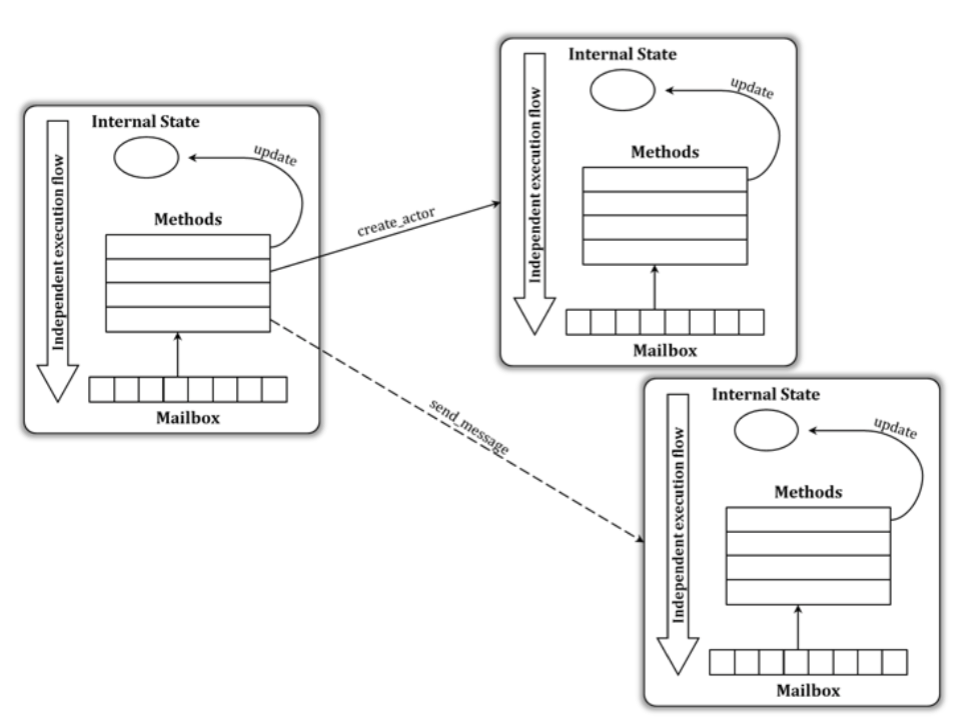
\includegraphics[scale=0.4]{images/analysis/Actor-model.png}
%\captionsetup{labelformat=empty}
\caption{Rappresentazione semplificata del modello ad attori}
\label{analisi-della-concorrenza-concorrenza-image-actor-model}
\end{figure}

La Figura \ref{analisi-della-concorrenza-concorrenza-image-actor-model} riassume quanto descritto circa la definizione del modello. E' possibile osservare gli elementi principali che lo costituiscono tra cui:

\begin{itemize}
\item{un proprio flusso di esecuzione indipendente dagli altri presenti;}
\item{le operazioni che esso può svolgere sul sistema come risultato dell'esecuzione di una particolare operazione.}
\end{itemize}

A conclusione della definizione del concetto di attore, è importante sottolineare che un attore \keyword{non condivide} con altri attori nel sistema il proprio stato interno, quindi per effettuare una modifica oppure ottenere informazioni in merito a tale stato è necessario inviare un esplicito messaggio all'attore interessato. E' opportuno inoltre specificare che l'ordine di arrivo dei messaggi, all'interno della \english{mailbox} di un attore, è del tutto indeterminato  a causa dell'asincronismo con cui essi sono inviati.

\subsection*{proprietà semantiche del modello}
\addcontentsline{toc}{subsection}{Proprietà semantiche del modello}
\label{analisi-della-concorrenza-concorrenza-proprietà-semantiche-del-modello}
Le proprietà semantiche chiave del modello ad attori sono:

\begin{itemize}
\item{incapsulamento dello stato interno;}
\item{atomicità d'esecuzione di ogni metodo come risposta ad un messaggio;}
\item{equità (\english{fairness}) nella gestione dell'avanzamento della computazione degli attori del sistema e nella consegna dei messaggi;}
\item{\english{location transparency}.}
\end{itemize}

\subsubsection*{incapsulamento}
La proprietà di incapsulamento (\english{encapsulation}) racchiude in sé quanto precedentemente detto nella definizione del concetto di attore circa il suo stato interno. Tale proprietà impone che due o più attori non possano condividere tra loro il proprio stato interno durante tutta l'esecuzione.

Volendo modificare o leggere lo stato interno di un attore, è necessario inviargli un esplicito messaggio ed attendere da lui una esplicita risposta.

Poiché il modello attori è intrinsecamente concorrente, è possibile che un messaggio giunga nella \english{mailbox} di un attore mentre quest'ultimo è impegnato nel processare un diverso messaggio giunto precedentemente nella \english{mailbox}\footnote{caso comune in caso di intensa attività}. Se per ipotesi fosse consentito, al secondo messaggio, di interrompere la gestione del primo per procedere all'immediata gestione del nuovo arrivato allora si otterrebbe come conseguenza che nel modello attori non sarebbe più possibile assumere che il comportamento di un attore, a fronte di un messaggio ricevuto, possa essere predeterminato in funzione del valore assunto dallo stato interno al momento della ricezione dello stesso.

\subsubsection*{atomicità}
La proprietà di atomicità (\english{atomicity}) evita la potenziale inconsistenza dello stato interno che si otterrebbe nel caso l'ipotesi effettuata nella sezione precedente circa l'eventuale assegnazione di livelli di priorità ai vari messaggi fosse verificata.

Nel modello ad attori, infatti, si impone che ciascun attore processi ogni messaggio in una unità atomica formata da tutte e sole le azioni necessarie atte a fornire una risposta al messaggio.

In tal modo si ottiene quindi una coda di esecuzione determinata dal momento di arrivo dei messaggi che permette di predeterminare il comportamento dell'attore a fronte dell'ordine di arrivo dei messaggi.

\subsubsection*{fairness}
La proprietà di \english{Fairness}\footnote{traducibile come ``equità e garanzia di esecuzione''} impone che ad ogni attore sia garantita la possibilità di computare se esso possiede almeno un messaggio a cui rispondere nella \english{mailbox}.

Impone inoltre che ogni messaggio inviato debba essere sempre consegnato all'attore destinatario con l'unica eccezione per quei messaggi destinati ad attori permanentemente o temporaneamente disabilitati nel sistema (attori impegnati in \english{loop} infiniti, che stanno tentando di eseguire un'operazione illecita oppure sono interdetti dalla ricezione di messaggi).

\subsubsection*{location transparency}
L'ultima proprietà semantica posseduta dal modello ad attori è la \english{location transparency}, ovvero la trasparenza rispetto alla dislocazione degli attori all'interno del sistema. 

Tale proprietà assicura l'importante caratteristica che consente ad un attore di non dipendere dalla posizione fisica all'interno del sistema. In questo modo un attore è in grado di scambiare messaggi con altri attori senza che esso sia a conoscenza del fatto che l'attore si trovi all'interno della stessa CPU o su un diverso computer collegato in rete dovendo di conseguenza impiegare tecniche di comunicazione differenti. Inoltre, mediante il rispetto di tale caratteristica, si ha la possibilità di effettuare una riconfigurazione del sistema in modo del tutto trasparente dalla logica di funzionamento.

L'indipendenza tra la locazione fisica e la locazione logica di ogni attore nel sistema, favorisce in tal senso un agile realizzazione di applicazioni distribuite.

\subsection*{stalli}
\addcontentsline{toc}{subsection}{Stalli}
\label{analisi-della-soluzione-concorrenza-stalli}
Dopo quanto illustrato sul modello ad attori è possibile notare come le uniche situazioni di stallo possibili si avrebbero solamente durante la fase di dialogo tra attori. Stallo possibile  in quanto ogni uno di essi possiede un unica risorsa \english{mailbox} la quale deve essere acceduta tramite mutua esclusione al fine di preservarne lo stato interno.

Al fine di evitare lo stallo si è deciso di invalidare la regola di Havender che sancisce l'accumulo di risorse, evitando quindi che un attore detenga l'accesso esclusivo a tali struttura dati quando debba comunicare con più attori.

\subsection*{viaggi fisicamente impossibili}
\addcontentsline{toc}{subsection}{Viaggi fisicamente impossibili}
\label{analisi-della-soluzione-concorrenza-viaggi-fisicamente-impossibili}
Attraverso l'implementazione del sistema secondo il modello ad attori la problematica riguardante viaggi fisicamente impossibili, illustrata nel precedente capitolo, risulta essere risolta direttamente dalle caratteristiche del modello stesso.

In particolare, la proprietà del modello che garantisce che tali viaggi non avvengano è l'atomicità. Ciò è vero perché nonostante un attore possa essere pre-rilasciato dal \english{runtime} sottostante tale pre-rilascio può avvenire solo in favore di un altro attore nel sistema; non è infatti possibile che la gestione di un messaggio venga interrotta in favore di un ulteriore messaggio, questo perché non esiste possibilità di avere messaggi con priorità differenti.

\section*{determinismo}
\addcontentsline{toc}{section}{Determinismo}
\label{analisi-della-soluzione-determinismo}
Il sistema oggetto di questa relazione presenta alcune parti che devono avere un comportamento \keyword{deterministico}.

Un comportamento deterministico deve essere osservato quando i veicoli giungono ad un incrocio stradale, esso deve consentire il suo attraversamento rispettando il codice stradale. La precedenza veicoli implementata è perciò la seguente:

\begin{enumerate}
\item{pedoni}
\item{autobus}
\item{automobili}
\end{enumerate}

Nell'implementazione attraverso il modello ad attori del sistema tale comportamento deterministico, lo si ottiene configurando appositamente le \keyword{\english{mailbox} degli attori} che personificano gli incroci cittadini.

L'algoritmo di \english{routing} implementato nel sistema presenta sia un comportamento deterministico che non deterministico. La componente deterministica dell'algoritmo impone che un percorso sia composto solamente da strade che interconnettono tra loro incroci consecutivi, mentre la componente non deterministica, e quindi non predicibile, riguarda il calcolo di un percorso per una destinazione, dovuta alla tecnica di \english{flooding} per l'inoltro dei messaggi di ricerca.

\section*{distribuzione}
\addcontentsline{toc}{section}{Distribuzione}
\label{analisi-della-soluzione-distribuzione}
Come precedentemente affermato quando la problematica/requisito di distribuzione è stata/o introdotta/o nel precedente capitolo, si è cercata una possibile suddivisione delle componenti del simulatore che però ne garantisse il corretto funzionamento.

Ad una prima analisi si può immaginare il simulatore composto delle seguenti macro componenti:

\begin{itemize}
\item{la città;}
\item{i veicoli (per il momento la tipologia non è influente);}
\item{i cittadini;}
\item{il monitor.}
\end{itemize}

Una componente per poter essere distribuita su più nodi deve essere \keyword{suddivisibile} in sotto-componenti di dimensione inferiore. Essa deve successivamente fornire un'interfaccia di accesso che non faccia trasparire all'esterno la sua distribuzione. In altre parole la componente deve apparire \keyword{compatta} e \keyword{coesa} alle componenti che la utilizzano, gestendo nel proprio stato interno la distribuzione.

Il \english{monitor} è un'entità quasi totalmente passiva in quanto il suo compito è solo quello di ricevere\footnote{non deve effettuare richieste specifiche se non al momento della connessione con il modulo \english{core} del simulatore.} eventi rilevanti e visualizzarli all'utente finale. Questa componente non presenta quindi i requisiti validi per una sua eventuale distribuzione.

Sia il veicolo che il cittadino sono entità molto piccole e passive e perciò non avrebbe alcun senso suddividerle all'interno di più nodi. Quindi anche queste ultime non presentano i requisiti fondamentali per una loro distribuzione.

La componente ``città'' è l'unica componente che è possibile scomporre in sotto-componenti senza che quest'ultima perda di significato. Quindi possiamo affermare che la città è suddivisibile in \keyword{quartieri}, ognuno dei quali composto da molteplici \keyword{incroci}. E' possibile suddividere ulteriormente la componente ``quartiere'' e distribuirne le sue sotto-componenti (gli incroci). Quest'ulteriore suddivisione in sotto-componenti può risultare utile in caso di quartieri densamente popolati di incroci, ma è tuttavia possibile spezzare questa moltitudine di incroci in più quartieri distinti mantenendosi cosi in linea con la progettazione. Si è perciò deciso di fermarsi alla suddivisione in quartieri.

Il sistema risulta perciò cosi distribuito nei diversi nodi della rete:

\begin{itemize}
\item{un nodo contenente l'attore ``città'', il quale funge come punto di accesso per l'intera struttura cittadina;}
\item{n nodi ognuno contenente un singolo attore ``quartiere''.}
\end{itemize}

Ogni incrocio conterrà invece informazioni utili alla costruzione dell'\keyword{overlay network},\footnote{rete virtuale che vive in cima alla rete reale che interconnette tra di loro i diversi nodi} rete, che a tutti gli effetti, fornisce forma alla città che si vuole simulare ed è formata da \keyword{collegamenti virtuali} tra i singoli quartieri che compongono tale città. Al fine dei instaurare tali collegamenti è necessario poter identificare univocamente ogni singolo incrocio che la compone, e per fare ciò si è adottata la convenzione di nomenclatura precedentemente illustrata.

\begin{figure}[h!]
\centering
\includegraphics[scale=0.5]{images/analysis/city-distribution.png}
\caption{Distribuzione delle componenti della città}
\label{analisi-della-soluzione-distribuzione-distribuzione-citta}
\end{figure}

In Figura \ref{analisi-della-soluzione-distribuzione-distribuzione-citta} è possibile osservare uno schema illustra la distribuzione di una città composta da 4 quartieri secondo quanto descritto in merito alla distribuzione delle componenti.

\subsection*{protocolli di comunicazione}
\addcontentsline{toc}{subsection}{Protocolli di comunicazione}
\label{analisi-della-soluzione-distribuzione-protocolli-di-comunicazione}
In seguito alla suddivisione delle componenti che compongono la città su diversi nodi è necessario istruire dei protocolli di comunicazione da utilizzarsi:

\begin{itemize}
\item{nella fase di inizializzazione (o \english{\keyword{bootstrap}}) del sistema;}
\item{nella fase di chiusura (o \english{\keyword{shutdown}}) del sistema.}
\end{itemize}

Data l'implementazione del sistema attraverso l'utilizzo del modello ad attori non è stato necessario considerare un \english{middleware} esterno per consentire la comunicazione tra le parti in quanto il modello espone la proprietà di \english{location transparency}.

\subsubsection*{protocollo di bootstrap}
Il protocollo di \english{bootstrap} risulta essere necessario in quanto è di fondamentale importanza che tutte le componenti siano create a pronte prima che la simulazione possa procedere. In particolare è necessario che tutte le componenti della città risultino essere presenti all'appello e che l'\english{overlay network} sia correttamente settata secondo quanto impostato nel file di configurazione del simulatore.

Gli attori che personificano sia la componente ``città'' che la componente ``distretto'' delegano ad un proprio attore la gestione locale delle fasi che compongono il protocollo di \english{bootstrap}. Esso ha come compito quello di reagire quando tutte le componenti, che la città o il quartiere devono amministrare, hanno confermato di aver completato la fase corrente di tale protocollo. Questo attore presenta un comportamento comune, sia che sia stia parlando dell'attore ``città'' che dell'attore ``distretto'', in quanto esso deve sollevare un evento al completamento di una fase. E' però necessario osservare che il comportamento adottato, al giungere dell'evento, è diverso nelle due componenti, quindi si sono implementati:

\begin{itemize}
\item{un \english{master bootstrap handler}\footnote{utilizzato dall'attore ``città''.}: il suo comportamento, al sollevamento dell'evento, ha come conseguenza un avanzamento alla prossima fase di \english{bootstrap}, la quale avviene attraverso l'invio esplicito di un messaggio agli attori a lui dipendenti;}
\item{uno \english{slave bootstrap handler}\footnote{utilizzato dall'attore ``distretto''.}: il suo comportamento, al sollevamento dell'evento, ha come conseguenza quella di informare l'attore immediatamente superiore in gerarchia che una fase è stata completa.}
\end{itemize}

Il protocollo di \english{boostrap} è composto dalle seguenti fasi che si susseguono una dopo l'altra:

\begin{enumerate}
\item{creazione locale delle componenti;}
\item{costruzione dell'\english{overlay network};}
\item{popolamento della città.}
\end{enumerate}

La prima fase del protocollo, creazione locale delle componenti, avviene non appena l'attore ``città'' riconosce e conferma il nuovo nodo che ha richiesto di partecipare nel sistema. Durante questa fase viene creato l'attore ``distretto'' (il quale funge da controllore o \english{controller} locale) che ha sua volta avvia la creazione degli incroci che dovrà amministrare durante lo svolgersi della simulazione.

Successivamente alla conferma ``di nascita'' di tutti i nodi che compongono la città quest'ultima avvia la seconda fase del protocollo, fase in cui viene costruita l'\english{overlay network}. Durante l'esecuzione, ogni incrocio utilizza le informazioni in suo possesso per creare dei collegamenti virtuali con gli incroci a lui vicini.

Infine, dopo la conferma che l'\english{overlay network} è stata settata, viene avviata l'ultima fase del protocollo: il popolamento. In questa fase l'attore ``città'', tramite l'invio di messaggi, popola quest'ultima con veicoli e persone che saranno utilizzati per animare la simulazione.

Al termine l'attore città comunica a tutte le sue componenti il segnale di ``start'' che avvierà la simulazione. Come si sarà sicuramente intuito la simulazione procede anche se non vi sono monitor che la osservano in quanto non si è ritenuto utile che fosse quest'ultima componente ad avviare il simulatore dato che la si è progettata per essere componente quasi totalmente passiva.

\subsection*{protocollo di shutdown}
Mentre le fasi del protocollo di \english{bootstrap} hanno la capacità di auto spiegarsi, non è altrettanto vero per lo \english{shutdown} del sistema. E' opportuno quindi descrivere il significato dell'asserzione ``l'applicazione ha terminato i propri compiti''. Si potrebbe ipotizzare che il sistema termini quando tutti gli attori vengono ad avere la loro \english{mailbox} vuota. Tale condizione presenta però i seguenti contro:

\begin{itemize}
\item{non è una condizione sufficiente alla terminazione di un attore poiché potrebbero esserci ulteriori attori, attualmente ``vivi'' nel sistema, che potrebbero voler inviare ancora messaggi a quest'ultimo;}
\item{non è una condizione verificabile data la natura del sistema, in quanto esso è progettato per procedere a ciclo continuo.}
\end{itemize} 

Il protocollo di \english{shutdown} progettato procede in modo del tutto analogo a quello di \english{bootstrap}, con la differenza che esso risulta essere composto da un unica fase. Anche in questo caso, sia l'attore ``città'' che l'attore ``distretto'' delegano ad un proprio attore la gestione dei questo protocollo, il quale ha un comportamento molto simile all'attore che gestisce la fasi del protocollo di \english{bootstrap}.

Gli attori che gestiscono il protocollo sono:

\begin{itemize}
\item{un \english{master shutdown handler}\footnote{utilizzato dagli attori ``città'' e ``distretto''.}: il suo comportamento, al sollevamento dell'evento, ha come conseguenza la chiusura del sistema locale;}
\item{uno \english{slave shutdown handler}\footnote{utilizzato dagli attori `incrocio''.}: il suo comportamento, al sollevamento dell'evento, ha come conseguenza la terminazione sicura dell'attore `incrocio'' stesso.}
\end{itemize}

\subsection*{recupero da fallimento}
\addcontentsline{toc}{subsection}{Recupero da fallimento}
\label{analisi-della-soluzione-distribuzione-recupero-da-fallimento}
E' opportuno corredare il \english{core} del simulatore di accorgimenti \english{software} che siano in grado di reagire ad eventuali fallimenti, siano essi \english{software} oppure provenienti dalla rete sui cui si appoggia il simulatore.

Gli accorgimenti da adottare includono:

\begin{itemize}
\item{l'esecuzione del sistema in \keyword{modalità supervisionata};}
\item{recuperare riferimenti agli attori.}
\end{itemize}

La modalità supervisionata consente, come per l'appunto il nome afferma, di supervisionare gli attori durante la loro esecuzione dotando il sistema di regole da adottarsi in caso di fallimento di uno di essi. Le tecniche adottabili consistono nel:

\begin{itemize}
\item{riprendere (\english{resume}) l'attore: in questo caso l'attore torna alle proprie mansioni come se nulla fosse accaduto, ma il messaggio che ha causato il fallimento viene scartato;}
\item{riavviare (\english{restart}) l'attore: in questo caso l'attore viene riavviato al fine di costruire una nuova istanza. Operazione desiderabile quando si ipotizza che lo stato interno dell'attore sia stato corrotto;}
\item{scalare (\english{escalate}) l'errore: in questo caso si delega la decisione sulla strategia da adottarsi all'attore più alto in grado nella gerarchia. Operazione adottabile qualora al livello in cui si trovi l'attore non si possiedano le informazioni necessarie a prendere una decisione;}
\item{fermare (\english{stop}) l'attore.}
\end{itemize}

Utilizzando le precedenti tecniche in accoppiata agli \english{hook} forniti dal ciclo di vita di un attore, illustrato in Figura \ref{analisi-del-problema-distribuzione-recupero-da-fallimento-ciclo-di-vita}, è possibile rendere il \english{core} del sistema tollerante ad eventuali guasti.

\begin{figure}
\centering
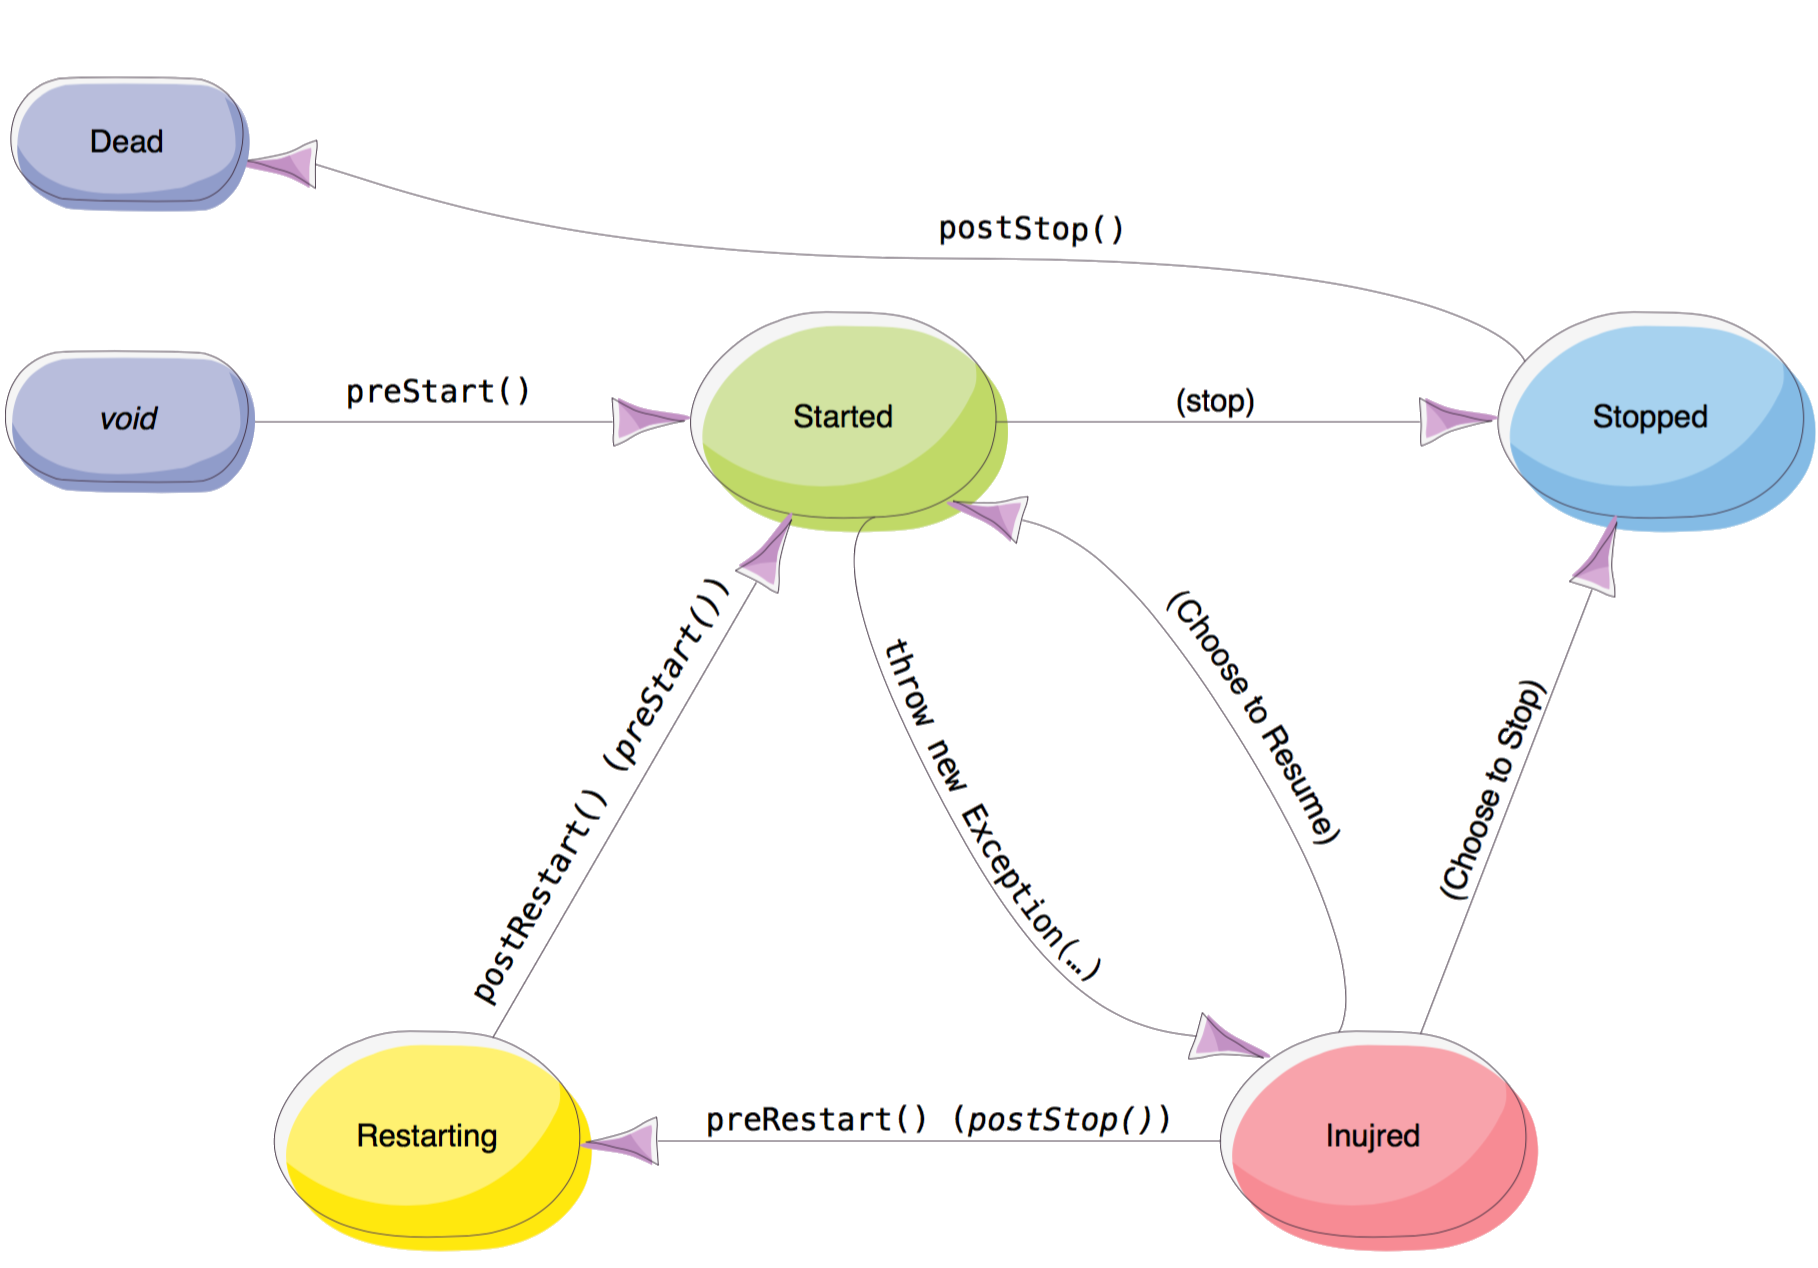
\includegraphics[scale=0.4]{images/analysis/Actor-lifecycle.png}
\caption{Ciclo di vita di un generico attore partecipante al sistema}
\label{analisi-del-problema-distribuzione-recupero-da-fallimento-ciclo-di-vita}
\end{figure}

Attraverso l'utilizzo di tali ``agganci'' è stato possibile conservare e successivamente passare i messaggi ancora nella \english{mailbox} alla nuova istanza dell'attore, nel caso in cui si fosse deciso di riavviarlo; oppure informare altri attori dell'avvenuto errore cosicché potessero attivare una procedura per il recupero del riferimento alla nuova istanza per poter continuare la simulazione.
%------------------------------------------------------------------------------
% solution.tex
%
% This illustrates the solution proposed. 
%------------------------------------------------------------------------------
\chapter*{soluzione proposta}
\addcontentsline{toc}{chapter}{Soluzione proposta}
\label{soluzione-proposta}
In questo capitolo sono fornite informazioni in merito alla soluzione proposta dallo studente.

\section*{tecnologie}
\addcontentsline{toc}{section}{Tecnologie}
\label{soluzione-proposta-tecnologie}
Per l'implementazione della soluzione proposta si sono utilizzate le seguenti tecnologie:

\begin{itemize}
\item{il linguaggio Scala con l'utilizzo delle librerie dell'Akka \english{framework} per l'implementazione del modulo ``\english{core}'' del sistema;}
\item{il linguaggio Scala con l'utilizzo del \english{Play framework} per l'implementazione del modulo ``monitor'' del sistema.}
\end{itemize}

\begin{figure}[h!]
\begin{subfigure}{0.5\textwidth}
\centering

\includegraphics[width=0.6\linewidth]{images/solution/scala.png}
\caption{Linguaggio Scala}
\end{subfigure}
\begin{subfigure}{0.5\textwidth}
\centering

\includegraphics[width=0.3\linewidth]{images/solution/akka.png}
\caption{Akka framework}
\end{subfigure}
\\
\begin{subfigure}{0.5\textwidth}
\centering

\includegraphics[width=0.3\linewidth]{images/solution/play.png}
\caption{Play framework}
\end{subfigure}
\begin{subfigure}{0.5\textwidth}
\centering

\includegraphics[width=0.4\linewidth]{images/solution/websocket.png}
\caption{web socket}
\end{subfigure}
\caption{Tecnologie utilizzate per il simulatore}
\label{soluzione-proposta-tecnologie-tecnologie-usate}
\end{figure}

L'utilizzo del linguaggio Scala si è preferito cosi da poter eseguire il simulatore su architetture differenti in quanto, l'eseguibile prodotto è formato da codice \english{bytecode} eseguibile sulle \ac{jvm}. Nonostante si basi sulla \ac{jvm} come \english{runtime} di esecuzione, si sono sfruttate le librerie del \english{framework} akka per l'utilizzo del modello ad attori per la gestione della concorrenza, un modello più valido rispetto alla gestione della concorrenza fornita dal linguaggio Java.

Come precedentemente affermato, data la proprietà di \english{location transparency} fornita dal modello ad attori non è stato necessario corredare il modulo \english{core} di un \english{middleware} esterno per la gestione delle comunicazioni tra i diversi nodi che lo compongono.

Infine si è scelto di utilizzare il \english{Play framework} per la costruzione di una \english{web application} che sia in grado di visualizzare lo stato corrente della simulazione. L'utilizzo di questa tecnologia e stato scelto poiché rende possibile il collegamento con il modulo \english{core} attraverso l'utilizzo di \english{web socket}. L'utilizzo di queste ultime consente la creazione di un canale \english{full-duplex} tra \english{client} e \english{server} che consente al  \english{core} di poter inviare eventi rilevanti alla grafica senza che quest'ultima esegua azioni di \english{polling} per rimanere aggiornata.

Lo svincolo dalla tecnica del \english{polling} consente di avere un sistema che sia in grado di reggere un numero molto superiore di \english{client} che necessitano di visualizzare lo stato della simulazione.

\section*{architettura del sistema}
\addcontentsline{toc}{section}{Architettura del sistema}
\label{soluzione-proposta-architettura}
In Figura \ref{soluzione-proposta-architettura-immagine} è visualizzato un diagramma di alto livello\footnote{Si vuole far notare al lettore che nel diagramma sono presenti, per semplicità, solo le connessioni più importanti} illustrante l'architettura del sistema costruito. Viene ora fornita una breve spiegazione degli attori principali che prendono parte al sistema.

\begin{figure}[h!]
\centering
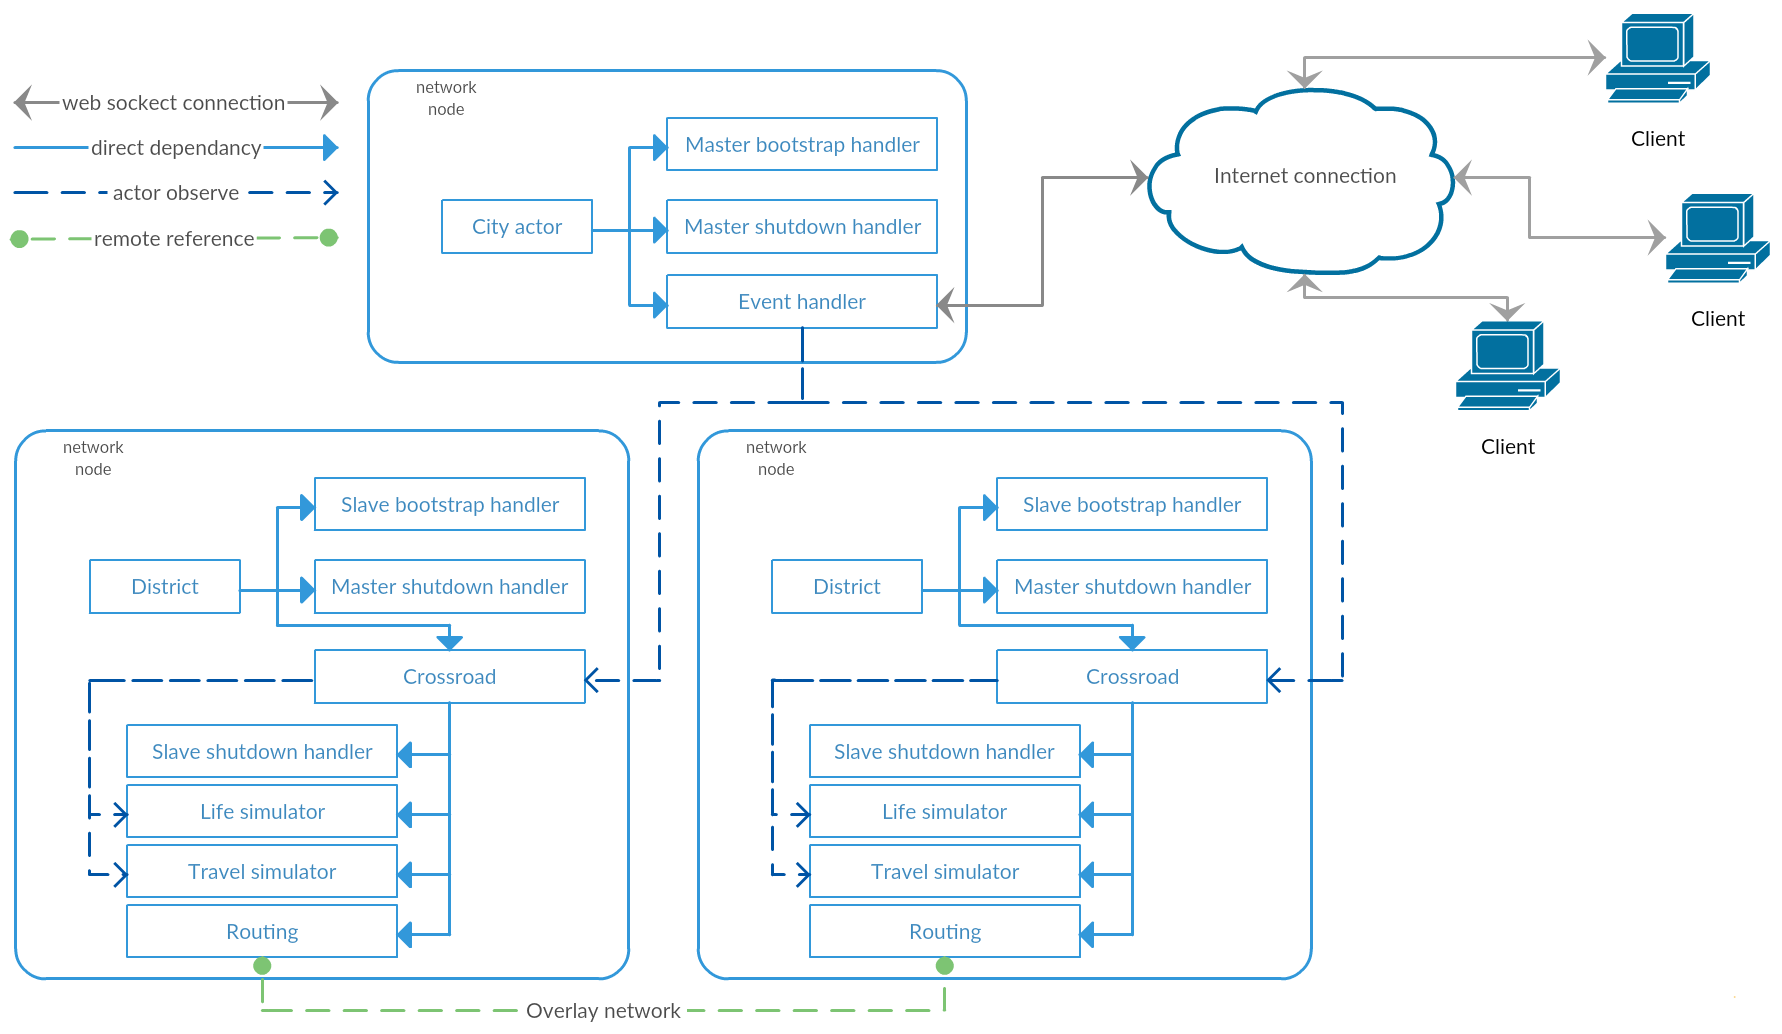
\includegraphics[scale=0.25]{images/solution/architecture.png}
\caption{Architettura del sistema}
\label{soluzione-proposta-architettura-immagine}
\end{figure}

\subsection*{attore ``city''}
\addcontentsline{toc}{subsection}{Attore ``city''}
\label{soluzione-propoposta-architettura-city}
L'attore amministra l'accesso alla struttura cittadina da parte dei \english{client} ed altre componenti che hanno necessità di dialogare con essa. E' composto dei seguenti attori, ai quali delega compiti specifici:

\begin{itemize}
\item{\english{MasterBootstrapHandler}: il quale gestisce le fasi del protocollo di \english{bootstrap} per l'intera struttura dati;}
\item{\english{MasterShutdownHandler}: il quale gestisce le fasi del protocollo di \english{shutdown} per l'intera struttura dati;}
\item{\english{EventHandler}: il quale riceve ed elabora gli eventi, provenienti dagli incroci, prima di inviarli ai \english{client}.}
\end{itemize}

\subsection*{attore ``master-bootstrap-handler''}
\addcontentsline{toc}{subsection}{Attore ``master-bootstrap-handler''}
\label{soluzione-poposta-architettura-master-bootstrap-handler}
L'attore amministra il \english{bootstrap} dei nodi che gestiranno i quartieri (o distretti) di cui è composta la città. Nel momento in cui esso rileva che l'\english{overlay network} è correttamente settata e che l'attore amministrante lo \english{shutdown} del sistema ha i riferimenti agli attori, esso termina le proprie mansioni cedendo il controllo all'attore ``Città'' per iniziare la fase di popolamento.

\subsection*{attore ``slave-bootstrap-handler''}
\addcontentsline{toc}{subsection}{Attore ``slave-bootstrap-handler''}
\label{soluzione-poposta-architettura-slave-bootstrap-handler}
L'attore amministra il \english{bootstrap} degli incroci che sotto la giurisdizione di un particolare distretto. Nel momento in cui esso rileva che la porzione di \english{overlay network}, gestita dal nodo stesso, è correttamente settata l'attore cessa le proprie mansioni comunicando all'attore ``distretto'' di rimanere in attesa dell'avvio della simulazione.

\subsection*{attore ``master-shutdown-handler''}
\addcontentsline{toc}{subsection}{Attore ``master-shutdown-handler''}
\label{soluzione-proposta-architettura-master-shutdown-handler}
L'attore amministra lo \english{shutdown} sia del nodo contenente l'attore ``città'' che il il nodo contenente l'attore ``distretto''. In particolare quando esso rileva che tutte gli attori di livello inferiore nella gerarchia, gli incroci nel caso degli attori ``distretti'' ed i distretti nel caso dell'attore ``città'', termina il sistema che gestisce e supervisiona gli attori. Come risultato finale si otterrà una chiusura sicura e pulita dell'intero sistema.

Nel caso di future espansioni del simulatore in questo punto è possibile inserire l'algoritmo di salvataggio dello stato del sistema, il quale verrà eseguito a simulazione interrotta e subito prima che il sistema cessi. Il salvataggio dello stato può avvenire implementando l'algoritmo dello \english{snapshot} distribuito determinato da Chandy e Lamport.

\subsection*{attore ``slave-shutdown-handler''}
\addcontentsline{toc}{subsection}{Attore ``slave-shutdown-handler''}
\label{soluzione-proposta-architettura-slave-shutdown-handler}
L'attore amministra lo \english{shutdown} di un singolo incrocio del sistema. Affinché tale attore possa terminare correttamente le proprie mansioni è necessario che gli attori a cui esso delega parte del lavoro di simulazione abbiano terminato le proprie mansioni.

\subsection*{attore ``event-handler''}
\addcontentsline{toc}{subsection}{Attore ``event-handler''}
\label{soluzione-proposta-architettura-event-handler}
L'attore ha il compito di registrarsi come ascoltatore di eventi presso gli incroci che costituiscono la città e di processarli, secondo esigenze specifiche, prima che essi siano inviati alla componente monitor. La traduzione degli eventi dallo stato ``grezzo'' allo stato ``lavorato'' viene delegata ad attori specifici per ogni tipologia di elaborazione a lui dipendenti che forniranno il risultato finale che verrà fornito alla componente monitor.

In Figura \ref{soluzione-proposta-architettura-event-handler-gerarchia} è visibile la gerarchia di attori eventi in carico la costruzione dei pacchetti dati da inviare alla componente ``monitor''. Gestendo, lato servente, tale tipo di computazione si ha la possibilità di costruire clienti più snelli e leggeri, potendo cosi supportare anche quelli con risorse limitate.

\begin{figure}[h!]
\centering
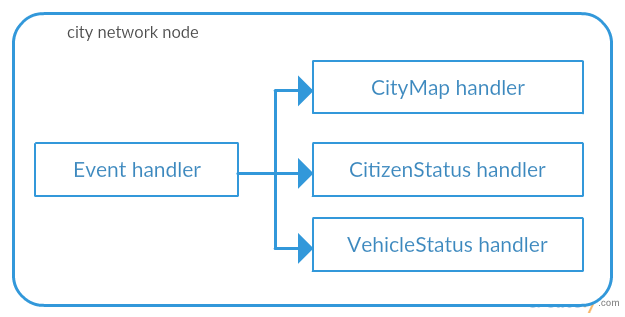
\includegraphics[scale=0.5]{images/solution/event-handler.png}
\caption{Attori aventi il compito della gestione degli eventi per la componente monitor}
\label{soluzione-proposta-architettura-event-handler-gerarchia}
\end{figure}

L'attore ``\english{CityMap handler}'' ha il compito di costruire un pacchetto dati contenente le informazioni che il \english{client} utilizza per visualizzare la mappa della struttura cittadina. Esso fornisce una struttura dati JSON contenente la gerarchia della componenti costituenti la città, ognuna di essa corredata con le coordinate geografiche che il \english{client} utilizzerà per visualizzare la mappa.

L'attore ``\english{CitizenStatus handler}'' ha il compito di costruire delle stringhe testuali che illustrino lo stato attuale di un cittadino nel sistema. Quest'ultimo può trovarsi in:

\begin{itemize}
\item{riposo (sta dormendo presso la propria abitazione);}
\item{alla fermata dell'autobus (se è previsto che esso debba viaggiare tramite un autobus);}
\item{in viaggio;}
\item{lavorando (sta eseguendo le proprie mansioni nel luogo di lavoro).}
\end{itemize}

L'attore ``\english{VehicleStatus handler}'' ha il compito di tradurre lo stato di avanzamento di un veicolo in coordinate geografiche valide relative alla mappa della città in questione.

\subsection*{attore ``district''}
\addcontentsline{toc}{subsection}{Attore ``district''}
\label{soluzione-proposta-architettura-district}
L'attore amministra l'accesso alle componenti che compongono il distretto da parte dell'attore ``city''.

\subsection*{attore ``crossroad''}
\addcontentsline{toc}{subsection}{Attore ``crossroad''}
\label{soluzione-proposta-architettura-crossroad}
L'attore è il vero artefice della simulazione in quanto consente ai veicoli di poter transitare nella città. Le azioni inerenti la simulazione vera e propria sono gestite da attori specifici a lui dipendenti, tra cui si può trovare:

\begin{itemize}
\item{\english{life simulator};}
\item{\english{travel simulator};}
\item{\english{routing}.}
\end{itemize}

Nelle sezioni successive viene fornita una breve descrizione del ruolo assunto da tali attori. Lo stato interno di tale attore contiene invece:

\begin{itemize}
\item{un \keyword{parcheggio} contenente i veicoli in attesa del segnale di avvio simulazione o di avere informazioni di \english{routing} per raggiungere una destinazione;}
\item{una \keyword{fermata dell'autobus}, la quale ospita le persone che attendono il passeggio dell'autobus o che, appena scese dal medesimo, si stanno per recare a compiere le proprie mansioni;}
\item{un \keyword{garage}, il quale contiene le automobili parcheggiate dai rispettivi proprietari mentre questi ultimi stanno compiendo le proprie mansioni.}
\end{itemize}

\subsection*{attore ``life simulator''}
\addcontentsline{toc}{subsection}{Attore ``life simulator''}
\label{soluzione-proposta-architettura-life-simulator}
L'attore consente ad un cittadino, giunto alla propria destinazione, di svolgere le proprie mansioni, in base alle sue esigenze, prima che questo possa riprendere il viaggio. Al momento la simulazione di lavoro/riposo avviene attraverso una sospensione ma è possibile inserire, in questo punto, l'implementazione di algoritmi specifici in base all'azione che ogni persona deve svolgere.

\subsection*{attore ``travel simulator''}
\addcontentsline{toc}{subsection}{Attore ``travel simulator''}
\label{soluzione-proposta-architettura-travel-simulator}
L'attore ha il compito di simulare il viaggio che un veicolo compie nel raggiungere un incrocio a lui immediatamente adiacente. Tale simulazione avviene utilizzando attraverso lo \english{scheduler}, fornito dalla libreria Akka, il quale consente di simulare avanzamenti progressivi e discreti nella strada che collega i due incroci.

Lo \english{scheduler} fornito con la libreria non rientra però nella categoria degli \english{scheduler real-time} in quanto l'implementazione standard si basa su \english{bucket} di lavoro, i quali sono svuotati secondo un calendario fissato. Ciò comporta che i compiti programmati non non sono eseguiti al momento esatto ma al primo \english{tick} immediatamente successivo al tempo programmato.

\subsection*{attore ``routing''}
\addcontentsline{toc}{subsection}{Attore ``routing''}
\label{soluzione-proposta-architettura-routing}
L'attore ha il compito di gestire l'\english{overlay network} che compone la struttura cittadina e di utilizzarla per determinare una strada, che parta dall'incrocio da cui esso dipende, verso una specifica destinazione utilizzando l'algoritmo di \english{routing} \ac{aodv}.

\section*{miglioramenti alla progettazione}
\addcontentsline{toc}{section}{Miglioramenti alla progettazione}
\label{soluzione-proposta-miglioramenti-alla-progettazione}
Alla luce di quanto esposto, in merito alle caratteristiche possedute dal modello ad attori, un possibile miglioramento consiste nell'evitare che gli attori ``\english{travel simulator}'' e ``\english{life simulator}'' gestiscano più mezzi e persone.

Si potrebbe invece delegare il compito della gestione dei viaggi e della simulazione della vita a copie dello stesso attore, creato nel momento del bisogno, che però gestiscano un singolo veicolo e una singola persona auto terminandosi al termine dello svolgimento del loro compito.

Introducendo nel sistema questa miglioria è compito dell'attore incrocio gestire, in una prima fase, la ricezione degli eventi prodotti da questi attori per poi inoltrarla agli attori interessati, tra cui ``\english{event handler}.

\section*{configurazione}
\addcontentsline{toc}{section}{Configurazione}
\label{soluzione-proposta-configurazione}
La configurazione del sistema avviene tramite la stesura di un file XML contenente le informazioni in merito alla struttura della città, delle persone che in essa vivono e dei mezzi di trasporto pubblici che per essa circolano.

La scelta di utilizzare il linguaggio XML è dovuta alla possibilità di utilizzare un'apposita grammatica durante la fase \english{unmarshalling} con cui è possibile verificare la bontà della configurazione fornita. Questo impedisce al sistema di avviarsi in caso di file non corretto, prevenendo cosi possibili errori che sicuramente sarebbero sollevati durante la fase di \english{bootstrap} del sistema o durante l'esecuzione della simulazione.

\section*{requisiti}
\addcontentsline{toc}{section}{Requisiti}
\label{soluzione-proposta-requisiti}
I requisiti del sistema sono:

\begin{itemize}
\item{una città, possibilmente configurabile prima dell'avvio del sistema;}
\item{un insieme configurabile di veicoli e persone che in essa circolano e svolgono le loro mansioni;}
\item{un sistema di controllo capace di visualizzare in tempo reale lo stato della simulazione.}
\end{itemize}

Il primo requisito è stato pienamente soddisfatto in quanto il sistema è in grado di leggere la struttura della città da un \english{file} di configurazione e di ricostruire in modo distribuito tale struttura secondo quanto precedentemente illustrato.

Anche il secondo requisito risulta pienamente soddisfatto in quanto è possibile configurare, sempre nel medesimo file di configurazione, un insieme variabile di mezzi e persone che opereranno nel sistema.

Per quanto riguarda l'ultimo requisito, esso risulta parzialmente soddisfatto in quanto si è stati solamente in grado di fornire una progettazione per una sua futura realizzazione e si è predisposto il modulo \english{core} per ospitarlo.

\section*{test eseguiti}
\addcontentsline{toc}{section}{Test eseguiti}
\label{soluzione-proposta-test-eseguiti}
Al fine di verificare si sono eseguiti i seguenti \english{test} sulle parti che compongono il sistema:

\begin{center}
\addcontentsline{lot}{table}{Elenco test eseguiti}
\begin{longtable}{| p{6cm} | p{7cm} |}
%\caption{test eseguiti}\\
%\label{soluzione-proposta-test-eseguiti-elenco}\\
\hline
\multicolumn{1}{| c |}{\textbf{Componente}} & \multicolumn{1}{ c |}{\textbf{\english{test}}}\\
\hline
\endfirsthead
\hline
\multicolumn{1}{| c |}{\textbf{Componente}} & \multicolumn{1}{ c |}{\textbf{\english{test}}}\\
\hline
\endhead
\english{Remote configuration} & \english{must setup correctly the underlying framework to operate with remote components}\\
\hline
\english{City car} & \english{must respect the planned travel}\\
\hline
& \english{must not change the programmed destination if the citizen status does not coincide with one of its tasks}\\
\hline
\english{City bus} & \english{must respects the planned stops}\\
\hline
& \english{must be empty when it starts the service in the city}\\
\hline
& \english{must not accept citizen that must travel with a different vehicle}\\
\hline
& \english{must be non empty when a citizen complete the boarding phase}\\
\hline
& \english{must be empty when the last passenger complete the landing phase}\\
\hline
& \english{must not permit that a citizen complete the boarding phase if it is already a bus passenger}\\
\hline
& \english{must have unchanged passengers list when it doing a not planned stop}\\
\hline
& \english{must have unchanged passengers list when it doing a planned stop and no one boarding or landing}\\
\hline
& \english{must let down only the passengers that have reached the correct bus stop}\\
\hline
& \english{must not contain passengers over its declared capacity}\\
\hline
\english{Pawn} & \english{must respect the planned travel}\\
\hline
& \english{must not change the programmed destination if the citizen status does not coincide with one of its tasks}\\
\hline
\english{ID generator} & \english{must generate keys with the correct length based on the number of critical components present in the system}\\
\hline
& \english{must generate chars in the specified interval}\\
\hline
\english{Address book} & \english{must be empty when it is created}\\
\hline
& \english{must permit the insertion of an address with the associated key}\\
\hline
& \english{must get the address associated to a key}\\
\hline
& \english{must be empty when it is cleaned}\\
\hline
& \english{must update the entry when an address with an existing key is inserted}\\
\hline
& \english{must get no data if it non contains the requested key}\\
\hline
& \english{must permit the deletion of an address and the associated key}\\
\hline
& \english{must remain unchanged when try to remove an address not present}\\
\hline
\english{Observable actor} & \english{must have no listeners registered when the actor is born}\\
\hline
& \english{must allow the registration of a new listener}\\
\hline
& \english{must not allow the registration of the same listener multiple times}\\
\hline
& \english{must allow the deletion of a listener}\\
\hline
& \english{must notify all the listeners if an event occurs}\\
\hline
\english{XML unmarshaller} & \english{must recognize a valid configuration file}\\
\hline
& \english{must recognize an invalid configuration file}\\
\hline
& \english{must not load an inexistent configuration file}\\
\hline
& \english{must correctly compute the number of components}\\
\hline
& \english{must correctly find the host addresses given the district name}\\
\hline
& \english{must create city objects according to the configuration file}\\
\hline
& \english{must correctly find the TCP port given the district name}\\
\hline
& \english{must create citizen objects according to the configuration file}\\
\hline
& \english{must create vehicle objects according to the configuration file}\\
\hline
\english{Routing table} & \english{must be empty when it is created}\\
\hline
& \english{must permit the insertion of a new route found by the algorithm}\\
\hline
& \english{must not contain routing information over its capacity}\\
\hline
& \english{must replace the older route information when there is no available place}\\
\hline
& \english{get the next hop information about and address memorized}\\
\hline
& \english{get no information about a destination if the address is not memorized in it}\\
\hline
& \english{be empty when it is cleaned} \\
\hline
& \english{permit to refresh the freshness of a route information}\\
\hline
& \english{permit the deletion of a route}\\
\hline
& \english{permit to update the information about a memorized route}\\
\hline
& \english{inser the route information if the update opration found that the route information does not exist in it}\\
\hline
\english{Travel actor} & \english{must correctly simulate the through of a stree that link two crossroad in the city}\\
\hline
& \english{must correctly manage the panned event when it shutting down}\\
\hline
\end{longtable}
\end{center}

Il test effettivo del sistema, invece, è stato eseguito analizzando il log prodotto dal simulatore durante la sua esecuzione e si è verificato che un veicolo procedesse solamente tra incroci consecutivi e che fosse in grado di raggiungere la destinazione prefissata. Si è inoltre osservato che la versione dell'algoritmo di \english{routing} implementato non sempre determina la strada più breve per giungere a destinazione.
%------------------------------------------------------------------------------
% conclusion.tex
%
% This illustrates the student conclusion. 
%------------------------------------------------------------------------------
\chapter*{conclusioni}
\addcontentsline{toc}{chapter}{Conclusioni}
\label{conclusioni}
L'opportunità di affrontare questo progetto ha fornito la possibilità di valutare molti aspetti inerenti al lavoro dello sviluppo \english{software}. Esso non ha ha riguardato solamente il singolo corso in sé ma ha consentito di riassumere conoscenze provenienti da altri corsi, seguiti anche durante lo svolgimento della Laurea Triennale.

Generalmente nello sviluppo \english{software} effettuato per altri corsi seguiti in precedenza, dato un obiettivo il fine ultimo consisteva solamente nel costruire un prototipo funzionante senza troppo preoccuparsi della correttezza delle scelta progettuali effettuate, cercando invece di adattarle man mano che il progetto evolveva. Con questo progetto ci si è imposti l'implementazione di \keyword{processi}, provenienti dal campo dell'ingegneria del \english{software}, che hanno sancito il seguente flusso di lavoro ciclico, a seguito di una fase di progettazione globale del sistema:

\begin{itemize}
\item{sviluppo della singola componente;}
\item{test di unità sulla componenti in casi comuni di utilizzo della medesima;}
\item{stesura della relativa documentazione, sia per il codice sorgente che per il codice di test.}
\end{itemize}

L'utilizzo di tale metodologia ha consentito di scoprire errori, inerenti alla progettazione, in fase d'implementazione delle singole componenti evitando cosi una grossa perdita di tempo dovuta alla gestione di molteplici errori rilevati nel momento dell'integrazione dell'intero sistema.

Infine, parlando di tecnologie, questo progetto mi ha consentito di vagliarne diverse prima di entrare nella fase dello sviluppo consentendo cosi una scelta delle stesse non basata sulla semplicità di utilizzo o sulla ``moda del momento'', ma bensì cercandone alcune che avessero in sé quelle caratteristiche che consentissero uno sviluppo agile del progetto.

% Glossary
%\clearpage{}
\printGlossary{FALSE}

%appendix
\begin{appendices}
\addcontentsline{toc}{chapter}{Articolo relativo ad AODV}
\includepdf[pages=-]{appendix-a.pdf}
\end{appendices}
\end{document}